\documentclass[12pt,a4paper]{article}
\usepackage{ugmath}
\usepackage{float}
\usepackage{placeins}
\usepackage [spanish]{babel}
\usepackage[labelfont=bf,labelsep=space]{caption}
\newcommand{\paren}[1]{\left( #1 \right)}
\newcommand{\alumno}{Ricardo León Martínez}
\newcommand{\materia}{Calculo Diferencia e Integral II}
\newcommand{\profesor}{Fernando Nuñez Medina}
\newcommand{\tarea}{Tarea 5}
\newcommand{\fecha}{6/3/2026}

\begin{document}
    \begin{center}
    {\large\textbf{UNIVERSIDAD DE GUANAJUATO}}\\[0.3cm]
    {\normalsize\textbf{DIVISIÓN DE CIENCIAS NATURALES Y EXACTAS}}\\
    {\normalsize\textbf{CAMPUS GUANAJUATO}}\\[1cm]

    {\Large\textbf{\tarea\ (\materia)}}\\[1cm]
    \end{center}

    \textbf{Nombre:} \alumno \hfill 
    \textbf{Fecha:} \fecha \hfill 
    \textbf{Calificación:} \rule{3cm}{0.4pt} \\[0.3cm]

    \begin{mdframed}[style=mdbluebox,frametitle={Ejercicio 1}]
        Prueba la proposición 12. \textbf{Sugerencia:} Toda partición $P=\{t_{0},\dots,t_{n}\}$ del intervalo $[a,b]$ genera una partición
        $Q=\{t_{0}-c,\dots,t_{n}-c\}$ del intervalo $[a-c,b-c]$ y viceversa.
    \end{mdframed}

    \begin{proof}
        Los subintervalos de $P$ son $[t_{i-1},t_{i}]$, mientras que los de $Q$ son
        $[t_{i-1}-c,t_{i}-c]$. Ademas $(t_{i}-c)-(t_{i-1}-c)=t_{i}-t_{i-1}$. Por lo tanto
        las longitudes de los subintervalos coinciden. Sea
        \begin{equation*}
            M_{i}=\sup\{f(x):x\in[t_{i-1},t_{i}]\},\qquad m_{i}=\inf\{f(x):x\in[t_{i-1},t_{i}]\}.
        \end{equation*}
        Para la función $g(x)=f(x+c)$ en el intervalo correspondiente tenemos
        \begin{equation*}
            \sup\{g(x):x\in[t_{i-1}-c,t_{i}-c]\}=\sup\{f(x):x\in[t_{i-1},t_{i}]\}=M_{i},
        \end{equation*}
        y análogamente
        \begin{equation*}
            \inf\{g(x):x\in[t_{i-1}-c,t_{i}-c]\}=m_{i}.
        \end{equation*}
        La suma superior de $f$ respecto a $P$ es
        \begin{equation*}
            U(f,P)=\sum_{i=1}^{n}M_{i}(t_{i}-t_{i-1}).
        \end{equation*}
        La suma superior de $g$ respecto a $Q$ es
        \begin{equation*}
            U(g,P)=\sum_{i=1}^{n}M_{i}((t_{1}-c)-(t_{i-1}-c)).
        \end{equation*}
        Pero
        \begin{equation*}
            (t_{i}-c)-(t_{i-1}-c)=t_{i}-t_{i-1}
        \end{equation*}
        Por lo que
        \begin{equation*}
            U(g,P)=U(f,P).
        \end{equation*}
        De manera análoga
        \begin{equation*}
            L(g,Q)=L(f,P).
        \end{equation*}
        Como las sumas superiores e inferiores coinciden, se tiene
        \begin{equation*}
            \inf_{P\in\mathcal{P}}U(f,P)=\inf_{Q\in\mathcal{P}}U(g,Q),\qquad \sup_{P\in\mathcal{P}}L(f,p)=\sup_{Q\in\mathcal{P}}L(g,Q).
        \end{equation*}
        Por lo tanto $f$ es integrable en $[a,b]$ si y solo si $g$ es integrable en $[a-c,b-c]$, y entonces
        \begin{equation*}
            \int_{a}^{b}f(x)dx=\int_{a-c}^{b-c}f(x+c)dx.
        \end{equation*}
    \end{proof}

    \begin{mdframed}[style=mdbluebox,frametitle={Ejercicio 2}]
        Calcula las siguientes integrales:
        \begin{enumerate}
            \item[(a)] $\displaystyle\int\frac{x}{x^{2}+1}dx$.
            \item[(b)] $\displaystyle\int\sin^{2}(x)\cos(x)dx$.
            \item[(c)] $\displaystyle\int\frac{x}{\sqrt{4-x^{2}}}dx$.
            \item[(d)] $\displaystyle\int\frac{x}{\sqrt{9+x^{2}}}dx$.
            \item[(e)] $\displaystyle\int\frac{x}{\sqrt{x^{2}-2}}dx$.    
        \end{enumerate}
    \end{mdframed}

    \begin{solucion}
        \begin{enumerate}
            \item[(a)] $\displaystyle\int\frac{x}{x^{2}+1}dx$.\\
            Hagamos $u=x^{2}+1$ y $du=2xdx$. Por lo tanto
            \begin{align*}
                \int\frac{x}{x^{2}+1}dx&=\frac{1}{2}\int\frac{1}{u}du\\
                &=\frac{1}{2}\ln(\abs{u})\\
                &=\frac{1}{2}\ln(\abs{x^{2}+1}).
            \end{align*}
            \item[(b)] $\displaystyle\int\sin^{2}(x)\cos(x)dx$.\\
            Hagamos $u=\sin(x)$ y $du=\cos(x)dx$. En consecuencia
            \begin{align*}
                \int\sin^{2}(x)\cos(x)dx&=\int u^{2}du\\
                &=\frac{1}{3}u^{3}\\
                &=\frac{1}{3}\sin^{3}(x)
            \end{align*}
            \item[(c)] $\displaystyle\int\frac{x}{\sqrt{4-x^{2}}}dx$.\\
            Sea $x=2\sin(\theta)$ y $dx=2\cos(\theta)d\theta$. Entonces $-2\cos(\theta)=-\sqrt{4-x^{2}}$. En
            consecuencia,
            \begin{align*}
                \int\frac{x}{\sqrt{4-x^{2}}}dx&=\int\frac{2\sin(\theta)}{\sqrt{4-4\sin^{2}(\theta)}}2\cos(\theta)d\theta\\
                &=\int\frac{2\sin(\theta)}{2\cos(\theta)}2\cos(\theta)d\theta\\
                &=\int2\sin(\theta)d\theta\\
                &=-2\cos(\theta)\\
                &=-\sqrt{4-x^{2}}.
            \end{align*}
            \item[(d)] $\displaystyle\int\frac{x}{\sqrt{9+x^{2}}}dx$.\\
            Sea $x=3\tan(\theta)$ y $dx=3\sec^{2}(\theta)d\theta$. Entonces $3\sec(\theta)=\sqrt{x^{2}+9}$. En consecuencia,
            \begin{align*}
                \int\frac{x}{\sqrt{9+x^{2}}}&=\int\frac{3\tan(\theta)}{\sqrt{9+9\tan^{2}(\theta)}}3\sec^{2}(\theta)d\theta\\
                &=\int\frac{3\tan(\theta)}{3\sec(\theta)}3\sec^{2}(\theta)d\theta\\
                &=3\int\tan(\theta)\sec(\theta)d\theta
            \end{align*}
            Ahora, hagamos $u=\sec(\theta)$ y $du=\sec(\theta)\tan(\theta)d\theta$. Por lo tanto
            \begin{align*}
                3\int\tan(\theta)\sec(\theta)d\theta&=\int du\\
                &=3u\\
                &=3\sec(\theta)\\
                &=\sqrt{x^{2}+9}.
            \end{align*}
            Así,
            \begin{equation*}
                \int\frac{x}{\sqrt{x^{2}+9}}dx=\sqrt{x^{2}+9}.
            \end{equation*}
            \item[(e)] $\displaystyle\int\frac{x}{\sqrt{x^{2}-2}}dx$.\\
            Sea $x=\sqrt{2}\sec(\theta)$ y $dx=\sqrt{2}\sec(\theta)\tan(\theta)d\theta$. Entonces $\sqrt{2}\tan(\theta)=\sqrt{x^{2}-2}$. En consecuencia,
            \begin{align*}
                \int\frac{x}{\sqrt{x^{2}-2}}dx&=\int\frac{\sqrt{2}\sec(\theta)}{\sqrt{2\sec^{2}(\theta)-2}}\sqrt{2}\sec(\theta)\tan(\theta)d\theta\\
                &=\int\frac{\sqrt{2}\sec(\theta)}{\sqrt{2}\tan(\theta)}\sqrt{2}\sec(\theta)\tan(\theta)d\theta\\
                &=\sqrt{2}\int\sec^{2}(\theta)d\theta\\
                &=\sqrt{2}\tan(\theta)\\
                &=\sqrt{x^{2}-2}.
            \end{align*}
        \end{enumerate}
    \end{solucion}

    \begin{mdframed}[style=mdbluebox,frametitle={Ejercicio 3}]
        Calcula la integral
        \begin{equation*}
            \int\frac{x^{2}+5x-14}{(x+4)(x^{2}+2)}dx.
        \end{equation*}
    \end{mdframed}

    \begin{solucion}
        Notemos que el integrando es una funcion racional propia, así que seguiremos el método citado para descomponerlo en fracciones simples.
        En este caso el denominador ya esta descompuesto en factores lineales y cuadraticos irreducibles. Por el factor $(x+4)$ la descomposición
        del integrando en fracciones simples incluye una fracción de la forma
        \begin{equation*}
            \frac{A}{x+4}
        \end{equation*}
        y por el factor $(x^{2}+2)$ la descomposición del integrando en fracciones simples incluye una fracción de la forma
        \begin{equation*}
            \frac{Bx+C}{x^{2}+2}
        \end{equation*}
        Así, la descomposición en fracciones simples es
        \begin{equation}
            \frac{x^{2}+5x-14}{(x+4)(x^{2}+2)}=\frac{A}{x+4}+\frac{Bx+C}{x^{2}+2}
        \end{equation}
        Notemos que $A,B$ y $C$ cumplen (1) si y solo si $A,B$ y $C$ cumplen que
        \begin{equation}
            x^{2}+5x-14=A(x^{2}+2)+(Bx+C)(x+4).
        \end{equation}
        Reexpresamos (2) como
        \begin{equation}
            x^{2}+5x-14=(A+B)x^{2}+(4B+C)x+(2A+4C).
        \end{equation}
        Puesto que dos polinomios son iguales si sus coeficientes son iguales, de (3) obtenemos que $A,B$ y $C$ satisfacen el sistema de ecuaciones
        \begin{align*}
            A+B=1\\
            4B+C=5\\
            2A+4C=-14
        \end{align*}
        cuya solución es $A=-1$, $B=2$ y $C=-3$. Por lo cual
        \begin{equation*}
            \frac{x^{2}+5x-14}{(x+4)(x^{2}+2)}=-\frac{1}{x+4}+\frac{2x-3}{x^{2}+2}
        \end{equation*}
        y, en consecuencia
        \begin{align*}
            \int\frac{x^{2}+5x-14}{(x+4)(x^{2}+2)}&=\int-\frac{1}{x+4}+\frac{2x-3}{x^{2}+2}dx\\
            &=-\int\frac{1}{x+4}dx+\int\frac{2x}{x^{2}+2}dx-3\int\frac{1}{x^{2}+2}dx\\
            &=-\ln(\abs{x+4})+\ln(\abs{x^{2}+2})-3\arctan(\frac{x}{\sqrt{2}}).
        \end{align*}
    \end{solucion}

    \begin{mdframed}[style=mdbluebox,frametitle={Ejercicio 4}]
        Considera las funciones $f:(0,1]\to\mathbb{R}$,$g:(0,1]\to\mathbb{R}$ y $h:(0,1]\to\mathbb{R}$ dadas por
        \begin{equation*}
            f(x)=\frac{1}{\sqrt{x}},\quad g(x)=\frac{1}{x}\text{ y }h(x)=\frac{1}{x^{2}}
        \end{equation*}
        \begin{enumerate}
            \item[(a)] Dibuja las graficas de $f,g$ y $h$.
            \item[(b)] Calcula el área bajó la gráfica de cada una de las funciones $f,g$ y $h$.  
        \end{enumerate}
    \end{mdframed}

    \begin{solucion}
        \begin{enumerate}
            \item[(a)] Dibuja las graficas de $f,g$ y $h$\\
            \begin{figure}[h]
                \centering
                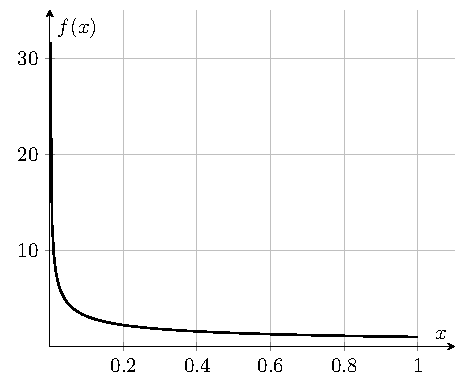
\includegraphics[width=0.32\textwidth]{f.pdf}
                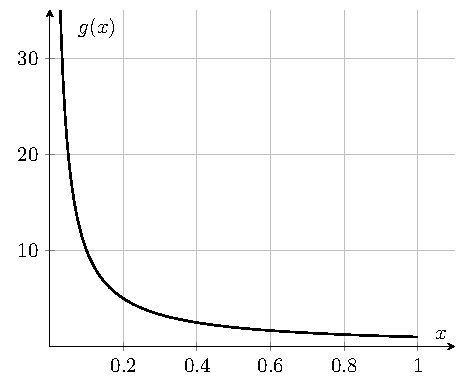
\includegraphics[width=0.32\textwidth]{g.pdf}
                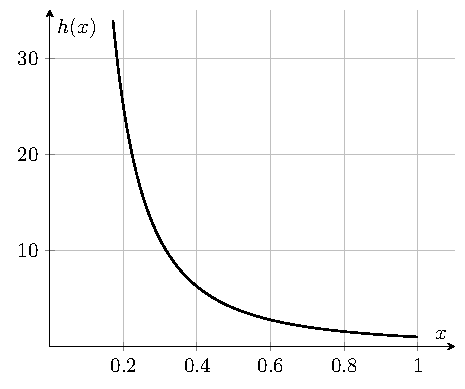
\includegraphics[width=0.32\textwidth]{h.pdf}
            \end{figure}
            \item[(b)] Calcula el área bajó la gráfica de cada una de las funciones $f,g$ y $h$.
            \begin{enumerate}
                \item[1.] $f(x)=\frac{1}{\sqrt{x}}$.\\
                El area bajo la gráfica de $f$ en el intervalo $(0,1]$ se describe mediante la integral impropia
                \begin{equation*}
                    \int_{0}^{1}\frac{1}{\sqrt{x}}dx,
                \end{equation*}
                la cual es impropia debido a que la función no está definida en $x=0$ y adémas
                \begin{equation*}
                    \lim_{x\to0^{+}}\frac{1}{\sqrt{x}}=+\infty.
                \end{equation*}
                Por definición de integral impropia en un extremo, se define
                \begin{equation*}
                    \int_{0}^{1}\frac{1}{\sqrt{x}}dx:=\lim_{t\to0^{+}}\int_{t}^{1}\frac{1}{\sqrt{x}}dx
                \end{equation*}
                Calculamos primero la integral $[t,1]$
                \begin{align*}
                    \int_{t}^{1}\frac{1}{\sqrt{x}}dx&=\int_{t}^{1}t^{-\frac{1}{2}}dt\\
                    &=\left[2x^{\frac{1}{2}}\right]_{t}^{1}\\
                    &=2-2t^{\frac12}
                \end{align*}
                Tomando el limite cuando $t\to0^{+}$
                \begin{equation*}
                    \int_{0}^{1}\frac{1}{\sqrt{x}}=\lim_{t\to0^{+}}2-2t^{\frac12}=2.
                \end{equation*}
                Así, el area bajo la grafica es 2
                \item[2.] $g(x)=\frac1x$\\
                El area bajo la gráfica de $f$ en el intervalo $(0,1]$ se describe mediante la integral impropia
                \begin{equation*}
                    \int_{0}^{1}\frac{1}{x}dx
                \end{equation*}
                la cual es impropia debido a que la función no está definida en $x=0$ y adémas
                \begin{equation*}
                    \lim_{x\to0^{+}}\frac1x=+\infty
                \end{equation*}
                Por definición de la integral impropio en un extremo, se define
                \begin{equation*}
                    \int_{0}^{1}\frac{1}{x}dx:=\lim_{t\to0^{+}}\int_{t}^{1}\frac{1}{x}dx
                \end{equation*}
                Calculamos primero la integral en $[t,1]$
                \begin{align*}
                    \int_{t}^{1}\frac1xdx&=\left[\ln(x)\right]_{t}^{1}\\
                    &=\ln(1)-\ln(t)\\
                    &=\ln(\frac1t)
                \end{align*}
                Tomando el limite cuando $t\to0^{+}$
                \begin{equation*}
                    \int_{0}^{1}\frac{1}{x}dx=\lim_{t\to0^{+}}\ln(\frac{1}{t})=+\infty
                \end{equation*}
                Así, el area bajo la gráfica diverge.
                \item[3.] $h(x)=\frac{1}{x^{2}}$\\
                El area bajo la gráfica de $f$ en el intervalo $(0,1]$ se describe mediante la integral impropia
                \begin{equation*}
                    \int_{0}^{1}\frac{1}{x^{2}}dx
                \end{equation*}
                la cual es impropia debido a que la función no está definida en $x=0$ y adémas
                \begin{equation*}
                    \lim_{x\to0^{+}}\frac{1}{x^{2}}=+\infty
                \end{equation*}
                Por definición de la integral impropio en un extremo, se define
                \begin{equation*}
                    \int_{0}^{1}\frac{1}{x^{2}}dx:=\lim_{t\to0^{+}}\int_{t}^{1}\frac{1}{x^{2}}dx
                \end{equation*}
                Calculamos primero la integral en $[t,1]$
                \begin{align*}
                    \int_{t}^{1}\frac{1}{x^{2}}dx&=\int_{t}^{1}x^{-2}\\
                    &=\left[-\frac{1}{x}\right]_{t}^{1}\\
                    &=-1+\frac{1}{t}
                \end{align*}
                Tomando el limite cuando $t\to0^{+}$
                \begin{equation*}
                    \int_{0}^{1}\frac{1}{x}dx=\lim_{t\to0^{+}}-1+\frac{1}{t}=+\infty
                \end{equation*}
                Así, el area bajo la gráfica diverge.
            \end{enumerate}
        \end{enumerate}
    \end{solucion}

    \begin{mdframed}[style=mdbluebox,frametitle={Ejercicio 5}]
        Calcula lo siguiente:
        \begin{enumerate}
            \item[(a)] El área entre las gráficas de las funciones $f(x)=x^{2}$ y $g(x)=1$ sobre el intevervalo
            $[-1,1]$.
            \item[(b)] El área entre las gráficas de las funciones $f(x)=\sin(x)$ y $g(x)=\cos(x)$ sobre el intervalo
            $[0,\pi]$.
        \end{enumerate}
    \end{mdframed}

    \begin{solucion}
        \begin{enumerate}
            \item[(a)] El área entre las gráficas de las funciones $f(x)=x^{2}$ y $g(x)=1$ sobre el intevervalo $[-1,1]$.\\
            Como $x^{2}\leq1$ en $[-1,1]$, entonces
            \begin{align*}
                A(f,g)&=\int_{-1}^{1}\abs{f-g}dx\\
                &=\int_{-1}^{1}(1-x^{2})dx\\
                &=\left[x-\frac{x^{3}}{3}\right]_{-1}^{1}\\
                &=\frac{2}{3}-\left(-\frac{2}{3}\right)\\
                &=\frac{4}{3}.
            \end{align*}
            \item[(b)] El área entre las gráficas de las funciones $f(x)=\sin(x)$ y $g(x)=\cos(x)$ sobre el intervalo
            $[0,\pi]$.
            Se resuelve
            \begin{equation*}
                \sin(x)=\cos(x).
            \end{equation*}
            Equivalentemente
            \begin{equation*}
                \tan(x)=1.
            \end{equation*}
            En el intervalo $[0,\pi]$ esto ocurre en
            \begin{equation*}
                x=\frac{\pi}{4}.
            \end{equation*}
            Ahora determinamos el orden. En $0\leq x\leq\frac{\pi}{4}$. Por ejemplo evaluando en $x=0$
            \begin{equation*}
                \sin(0)=0,\qquad\cos(0)=1.
            \end{equation*}
            Luego $\cos(x)\lt\sin(x)$. En $\frac{\pi}{4}\lt x\leq\pi$. Por ejemplo en $x=\frac{\pi}{2}$
            \begin{equation*}
                \sin(\frac{\pi}{2})=1,\qquad\cos(\frac{\pi}{2})=0.
            \end{equation*}
            Luego $\sin(x)\gt\cos(x)$. Por lo tanto el intervalo debe partirse en dos
            \begin{equation*}
                [0,\pi]=[0,\frac{\pi}{4}]\cup[\frac{\pi}{4},\pi].
            \end{equation*}
            De esta forma el area es
            \begin{align*}
                A(f,g)&=\int_{0}^{\frac{\pi}{4}}(\cos(x)-\sin(x))dx+\int_{\frac{\pi}{4}}^{\pi}(\sin(x)-\cos(x))dx.\\
                &=\big[\sin(x)+\cos(x)\big]_{0}^{\frac{\pi}{4}}+\big[-\cos(x)-\sin(x)\big]_{\frac{\pi}{4}}^{\pi}\\
                &=(\sqrt{2}-1)+(1+\sqrt{2})\\
                &=2\sqrt{2}.
            \end{align*}
        \end{enumerate}
    \end{solucion}

    \begin{mdframed}[style=mdbluebox,frametitle={Ejercicio 6}]
        Muestra que la longitud de la circunferencia con centro en el origen  y radio $r$ es $2\pi r$.
    \end{mdframed}

    \begin{proof}
        Sea
        \begin{equation*}
            f(x)=\sqrt{r^{2}-x^{2}}.
        \end{equation*}
        Entonces
        \begin{equation*}
            f^{\prime}(x)=\frac{1}{2}(r^{2}-x^{2})^{-\frac12}(-2x)=\frac{-x}{\sqrt{r^{2}-x^{2}}}.
        \end{equation*}
        Por lo tanto
        \begin{equation*}
            (f^{\prime}(x))^{2}=\frac{x^{2}}{r^{2}-x^{2}}.
        \end{equation*}
        Así, por la proposición 18, la longitud de arco es
        \begin{equation*}
            L=\int_{-r}^{r}\sqrt{1+\frac{x^{2}}{r^{2}-x^{2}}}dx.
        \end{equation*}
        Simplificando el integrando
        \begin{equation*}
            1+\frac{x^{2}}{r^{2}-x^{2}}=\frac{r^{2}-x^{2}+x^{2}}{r^{2}-x^{2}}=\frac{r^{2}}{r^{2}-x^{2}}.
        \end{equation*}
        Por lo tanto
        \begin{equation*}
            \sqrt{1+(f^{\prime}(x))}=\frac{r}{\sqrt{r^{2}-x^{2}}}.
        \end{equation*}
        Así,
        \begin{align*}
            L=\int_{-r}^{r}\frac{r}{\sqrt{r^{2}-x^{2}}}dx&=\big[r\arcsin(\frac{x}{r})\big]_{-r}^{r}
        \end{align*}
        Entonces
        \begin{equation*}
            \arcsin(1)=\frac{\pi}{2},\qquad \arcsin(-1)=-\frac{\pi}{2}.
        \end{equation*}
        Por lo tanto,
        \begin{equation*}
            L=r(\frac{\pi}{2}-(-\frac{\pi}{2}))=r\pi.
        \end{equation*}
        Así, hemos calculado la longitud de una semicircunferencia. La circunferencia completa
        es el doble de la semicircunferencia así,
        \begin{equation*}
            L_{circ}=2L=2\pi r.
        \end{equation*}
    \end{proof}

    \begin{mdframed}[style=mdbluebox,frametitle={Ejercicio 7}]
        Utiliza la circunferencia trigonometrica para calcular, si es que existe, el valor de las funciones trigonometricas del angulo
        $\theta$ de cada uno de los incisos siguientes (haz un dibujo).
        \begin{multicols}{2}
            \begin{enumerate}
                \item[(a)]  $\theta=\pi.$
                \item[(b)]  $\theta=3\pi/2.$
                \item[(c)]  $\theta=2\pi.$
                \item[(d)]  $\theta=-\pi/2.$
            \end{enumerate}
        \end{multicols}
    \end{mdframed}

    \begin{solucion}
        \begin{enumerate}
            \item[(a)] $\theta=\pi$.\\
            En la circunferencia trigonometrica el ángulo $\pi$ corresponde al punto $(-1,0)$.
            Por lo tanto
            \begin{equation*}
                \sin(\pi)=0, \qquad \cos(\pi)=1.
            \end{equation*}
            De aquí
            \begin{equation*}
                \tan(\pi)=\frac{0}{-1}=0,\\
                \sec(\pi)=-1,
            \end{equation*}
            mientras que $\csc(\pi)$ y $\cot(\pi)$ no existen, pues $sin(\pi)=0$.
            \begin{center}
                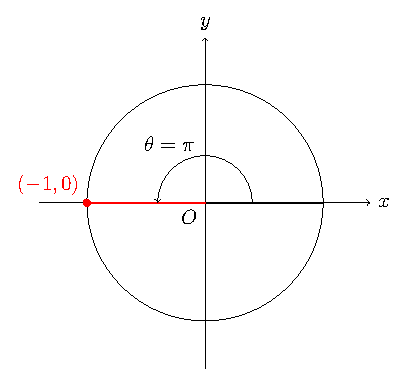
\includegraphics[width=0.35\textwidth]{a.pdf}
            \end{center}
            \item[(b)] $\theta=3\pi/2$.\\
            El angulo corresponde al punto $(0,-1)$. Por lo tanto
            \begin{equation*}
                \sin(\frac{3\pi}{2})=-1,\qquad \cos(\frac{3\pi}{2})=0.
            \end{equation*}
            Entonces $\tan(\frac{3\pi}{2})$ no existe. Además
            \begin{equation*}
                \csc(\frac{3\pi}{2})=-1
            \end{equation*}
            Mientras que
            \begin{equation*}
                \sec(\frac{3\pi}{2})\qquad\cot(\frac{3\pi}{2})
            \end{equation*}
            no existen.
            \begin{center}
                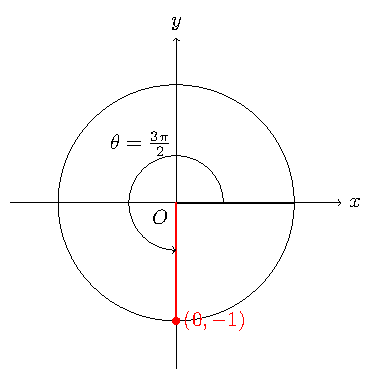
\includegraphics[width=0.35\textwidth]{b.pdf}
            \end{center}
            \item[(c)] $\theta=2\pi$.\\
            Este ángulo corresponde al punto $(1,0)$. Entonces
            \begin{equation*}
                \sin(2\pi)=0,\qquad \cos(2\pi)=1.
            \end{equation*}
            Por lo tanto
            \begin{equation*}
                \tan(2\pi)=0, \qquad \sec(2\pi)=1.
            \end{equation*}
            y $\csc(2\pi)$, $\cot(2\pi)$ no existen.
            \begin{center}
                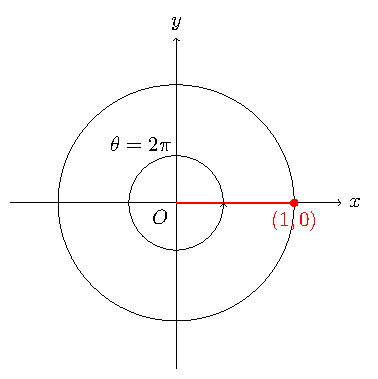
\includegraphics[width=0.35\textwidth]{c.pdf}
            \end{center}
            \item[(d)] $\theta=-\frac{\pi}{2}$.\\
            Este angulo representa una rotacion en sentido horario, cuyo punto es $(0,-1)$.
            Por lo tanto
            \begin{equation*}
                \sin(-\frac{\pi}{2})=-1,\qquad\cos(-\frac{\pi}{2})=0.
            \end{equation*}
            de aqui $\tan(-\frac{\pi}{2})$ no existe, mientras que
            \begin{equation*}
                \sec(-\frac{\pi}{2}),\qquad\cot(-\frac{\pi}{2})
            \end{equation*}
            no existen.
            \begin{center}
                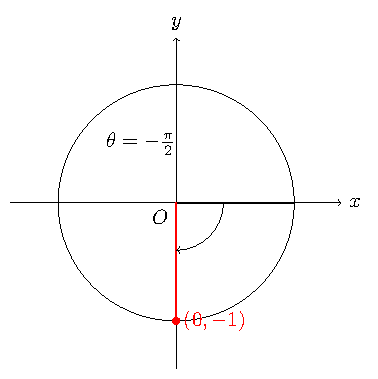
\includegraphics[width=0.35\textwidth]{d.pdf}
            \end{center}
        \end{enumerate}
    \end{solucion}

    \begin{mdframed}[style=mdbluebox,frametitle={Ejercicio 8}]
        Prueba los incisos (c) al (f) de la proposición 23.
    \end{mdframed}

    \begin{proof}
        \begin{enumerate}
            \item[(c)] $\tan^{\prime}(x)=\sec^{2}(x)$\\
            Sea $\tan(x)=\dfrac{\sin(x)}{\cos(x)}$. Utilizando la regla del cociente,
            \[
            \tan'(x)
            =
            \frac{\cos(x)\cos(x)-\sin(x)(-\sin(x))}{\cos^2(x)}.
            \]
            Simplificando,
            \[
            \tan'(x)
            =
            \frac{\cos^2(x)+\sin^2(x)}{\cos^2(x)}.
            \]
            Usando la identidad pitagórica $\sin^2(x)+\cos^2(x)=1$,
            \[
            \tan'(x)=\frac{1}{\cos^2(x)}=\sec^2(x).
            \]
            \item[(d)] $\cot^{\prime}(x)=-\csc^{2}(x)$\\
            Sea $\cot(x)=\dfrac{\cos(x)}{\sin(x)}$. Aplicando nuevamente la regla del cociente,
            \[
            \cot'(x)
            =
            \frac{(-\sin(x))\sin(x)-\cos(x)\cos(x)}{\sin^2(x)}.
            \]
            Simplificando,
            \[
            \cot'(x)
            =
            \frac{-\sin^2(x)-\cos^2(x)}{\sin^2(x)}.
            \]
            Usando $\sin^2(x)+\cos^2(x)=1$,
            \[
            \cot'(x)=-\frac{1}{\sin^2(x)}=-\csc^2(x).
            \]
            \item[(e)] $\sec^{\prime}(x)=\sec(x)\tan(x)$.\\
            Sea $\sec(x)=\dfrac{1}{\cos(x)}$. Entonces
            \[
            \sec'(x)
            =
            \frac{d}{dx}\left(\cos(x)^{-1}\right).
            \]
            Aplicando la regla de la cadena,

            \[
            \sec'(x)
            =
            -\cos(x)^{-2}(-\sin(x)).
            \]
            Por lo tanto
            \[
            \sec'(x)=\frac{\sin(x)}{\cos^2(x)}.
            \]
            Reescribiendo en términos de funciones trigonométricas,
            \[
            \sec'(x)
            =
            \frac{1}{\cos(x)}\frac{\sin(x)}{\cos(x)}
            =
            \sec(x)\tan(x).
            \]
            \item[(f)] $\csc^{\prime}(x)=-\csc(x)\cot(x)$.\\
            Sea $\csc(x)=\dfrac{1}{\sin(x)}$. Entonces
            \[
            \csc'(x)
            =
            \frac{d}{dx}\left(\sin(x)^{-1}\right).
            \]
            Aplicando la regla de la cadena,
            \[
            \csc'(x)
            =
            -\sin(x)^{-2}\cos(x).
            \]
            Por lo tanto
            \[
            \csc'(x)
            =
            -\frac{\cos(x)}{\sin^2(x)}.
            \]
            Reescribiendo,
            \[
            \csc'(x)
            =
            -\frac{1}{\sin(x)}\frac{\cos(x)}{\sin(x)}
            =
            -\csc(x)\cot(x).
            \]
        \end{enumerate}
    \end{proof}
\end{document}